\begin{enumerate}

\item 
\begin{enumerate}
	\item The two equilibria are $v = 0$ and 
	\begin{align*}
	pv^a - qv^b = 0 
		& \Leftrightarrow pv^a = qv^b \\	
		& \Leftrightarrow \frac{p}{q}= v^{b-a} \\
		& \Leftrightarrow v = \left(\frac{p}{q}\right)^{\frac{1}{b-a}} = v^\star
	\end{align*}

	We can study the stability of these equilibria by sketching the 1D phase portrait:
	
	\begin{center}
		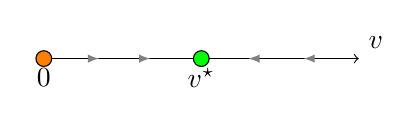
\begin{tikzpicture}
			\draw[->] (0,0) -- (4,0) node[above right] {$v$};
	%		\draw (0,0.1) -- (0,-0.1) ;
			\draw[fill=orange] (0,0) node[below] {$0$} circle (0.1);
	%		\draw (2,0.1) -- (2,-0.1) ;
			\draw[fill=green] (2,0) node[below] {$v^\star$} circle (0.1);
			\draw[-latex, gray] (0.69,0) -- (0.7,0);
			\draw[-latex, gray] (1.34,0) -- (1.35,0);		
			\draw[-latex, gray] (3.35,0) -- (3.3,0);
			\draw[-latex, gray] (2.65,0) -- (2.6,0);
		\end{tikzpicture}
	\end{center}

	We can deduce that:
	\begin{itemize}
		\item $v=0$ is unstable
		\item $v=v^\star$ is stable
	\end{itemize}
	
	
	
	\item From the phase portrait of the previous part, we can tell that the solutions are going to be monotonic:
	\begin{itemize}
		\item If $v_0 < v^\star$, then the tumour will increase monotonically
		\item If $v_0 > v^\star$, then the tumour will decrease monotonically
	\end{itemize}
	
	
	\item 
	\begin{align*}
	S(v^\star,p) 
		& = \frac{\partial v^\star}{\partial p} \frac{p}{v^\star} \\
		& = \frac{1}{q} \frac{1}{b-a} \left(\frac{p}{q}\right)^{\frac{1}{b-a}-1} \frac{p}{\left(\frac{p}{q}\right)^{\frac{1}{b-a}}} \\
		& = \frac{1}{b-a}
	\end{align*}
	
	So the sensitivity depends only on the difference between $a$ and $b$ and not on $p$ or $q$.
	
	
	\item This means that $qv^b = K N$, where $N$ is the number of cells. If the cells are all uniform, then the number of cells should be proportional to the volume, so we get $qv^b = k v$ and $b_0=1$.
	
	\item This implies $pv^a = K A$, where $A$ is the surface area.
	
	Then we have $v = k_1 r^3$ and $A = k_2 r^2$, where $r$ is the radius of the area occupied by the tumour. This implies that $ A = k_3  v^{2/3}$, so $pv^a = K v^{2/3}$, thus $a_0 = 2/3$.
	
	\item Since the tumour is increasing, we can deduce that its size will approach $v^\star$:
	\[
	v^\star 
		= \left(\frac{p}{q}\right)^{\frac{1}{b-a}} 
		= \left(\frac{0.72}{0.036}\right)^{\frac{1}{1-2/3}}
		= 8000 {\rm mm}^3 = 8 {\rm cm}^3
	\]
	
	We have data until the tumour reached the size of 4000 mm$^3$, or about half of our long term prediction, so our extrapolation is well outside the data we have. It is not very trustworthy.

	\end{enumerate}
	
	
	
	
\item 
\begin{enumerate}
	\item The quantity $Q$ represents the total number of cars in the highway.
	
	We have
	\begin{align*}
		\frac{d Q}{dt}
			& = \int_{-\infty}^{\infty} \frac{\partial \rho_1}{\partial t} + \frac{\partial \rho_2}{\partial t} ~dx \\
			& = \int_{-\infty}^{\infty} - \frac{\partial}{\partial x} \left[ \rho_1 v_{\max}(1-\rho_1/\rho_{\max})\right] - \frac{\partial}{\partial x} \left[ \rho_2 v_{\max}(1-\rho_2/\rho_{\max})\right] ~dx\\
			& = \lim_{x \to -\infty} \left\{ \frac{\partial}{\partial x} \left[ \rho_1 v_{\max}(1-\rho_1/\rho_{\max})\right] + \frac{\partial}{\partial x} \left[ \rho_2 v_{\max}(1-\rho_2/\rho_{\max})\right] \right\} \\
			& 	\qquad - \lim_{x \to +\infty} \left\{ \frac{\partial}{\partial x} \left[ \rho_1 v_{\max}(1-\rho_1/\rho_{\max})\right] + \frac{\partial}{\partial x} \left[ \rho_2 v_{\max}(1-\rho_2/\rho_{\max})\right] \right\} \\
			& = 0
	\end{align*}

	\item These terms represent cars changing lanes. When lane 1 has more cars than lane 2, then $\rho_1>\rho_2$ and $\alpha(\rho_2-\rho_1) <0$ meaning cars are leaving lane 1 to go to lane 2. This seems to be a reasonable way to model cars changing lanes.
	
	\item This means that at $x=2$, there should be an influx of cars added to the ``lane-changing-term''.
	
	Also, usually the cars join the right-most lane, so assuming that lane 1 is the right-lane and lane 2 is the left-lane, we get a new equation 1:
		\begin{equation}\label{entrance1}\tag{$S_1$}			
		\frac{\partial \rho_1}{\partial t} + \frac{\partial}{\partial x} \left[ \rho_1 v_{\max}(1-\rho_1/\rho_{\max})\right] = 	\alpha (\rho_2 - \rho_1) + n(t)\underbrace{\big(H_{2.5}(x)-H_{3.5}(x)\big)}_{\text{uniformly in }[2.5, 3.5]}
		\end{equation}
		where $H_a(x)$ is the Heaviside function.
		
		Alternatively we could have
		\begin{equation}\label{entrance2}\tag{$S_2$}			
		\frac{\partial \rho_1}{\partial t} + \frac{\partial}{\partial x} \left[ \rho_1 v_{\max}(1-\rho_1/\rho_{\max})\right] = 	\alpha (\rho_2 - \rho_1) + n(t)\underbrace{\frac{1}{\sqrt{\frac{\pi}{8}}}e^{-8(x-3)^2}}_{\substack{\text{normally distributed}\\\text{around $x=3$ with $\sigma=\frac14$}}}
		\end{equation}

		In this case, since cars are coming in, I expect that $Q$ will be increasing. In fact:
		\[
		\frac{dQ}{dt} = n(t) > 0,
		\]
		which means that the total number of cars in the highway will keep increasing by $n(t)$.
	
\end{enumerate}


\end{enumerate}